\documentclass[tikz,border=6pt]{standalone}
\usetikzlibrary{arrows.meta,positioning,calc,fit}
\makeatletter
\AtBeginDocument{\global\let\pgf@selectfontorig\relax}
\makeatother

\tikzset{
  state/.style={
    draw=black,
    rounded corners=4pt,
    very thick,
    fill=white,
    minimum width=8.5mm,
    minimum height=7mm,
    align=center,
    inner sep=1.6pt,
    font=\scriptsize
  },
  initial/.style={-Latex, very thick},
  edge/.style={-Latex, thick, shorten >=2pt, shorten <=2pt},
  labelbox/.style={inner sep=3pt, font=\tiny, scale=0.62, transform shape, align=center},
  panel/.style={draw=gray!70, rounded corners=6pt, very thick},
  title/.style={fill=white, inner sep=1.5pt, font=\itshape\large}
}

\newcommand{\initarrow}[2]{\draw[initial] #1 to (#2);}

\newcommand{\panel}[3]{
  \draw[panel] (-1.65,-2.65) rectangle (5.85,2.25);
  \ifdefined\qoption
  \else
  \node[title, anchor=north west] at (-1.55,2.15) {$#3$};
  \fi
}

\begin{document}
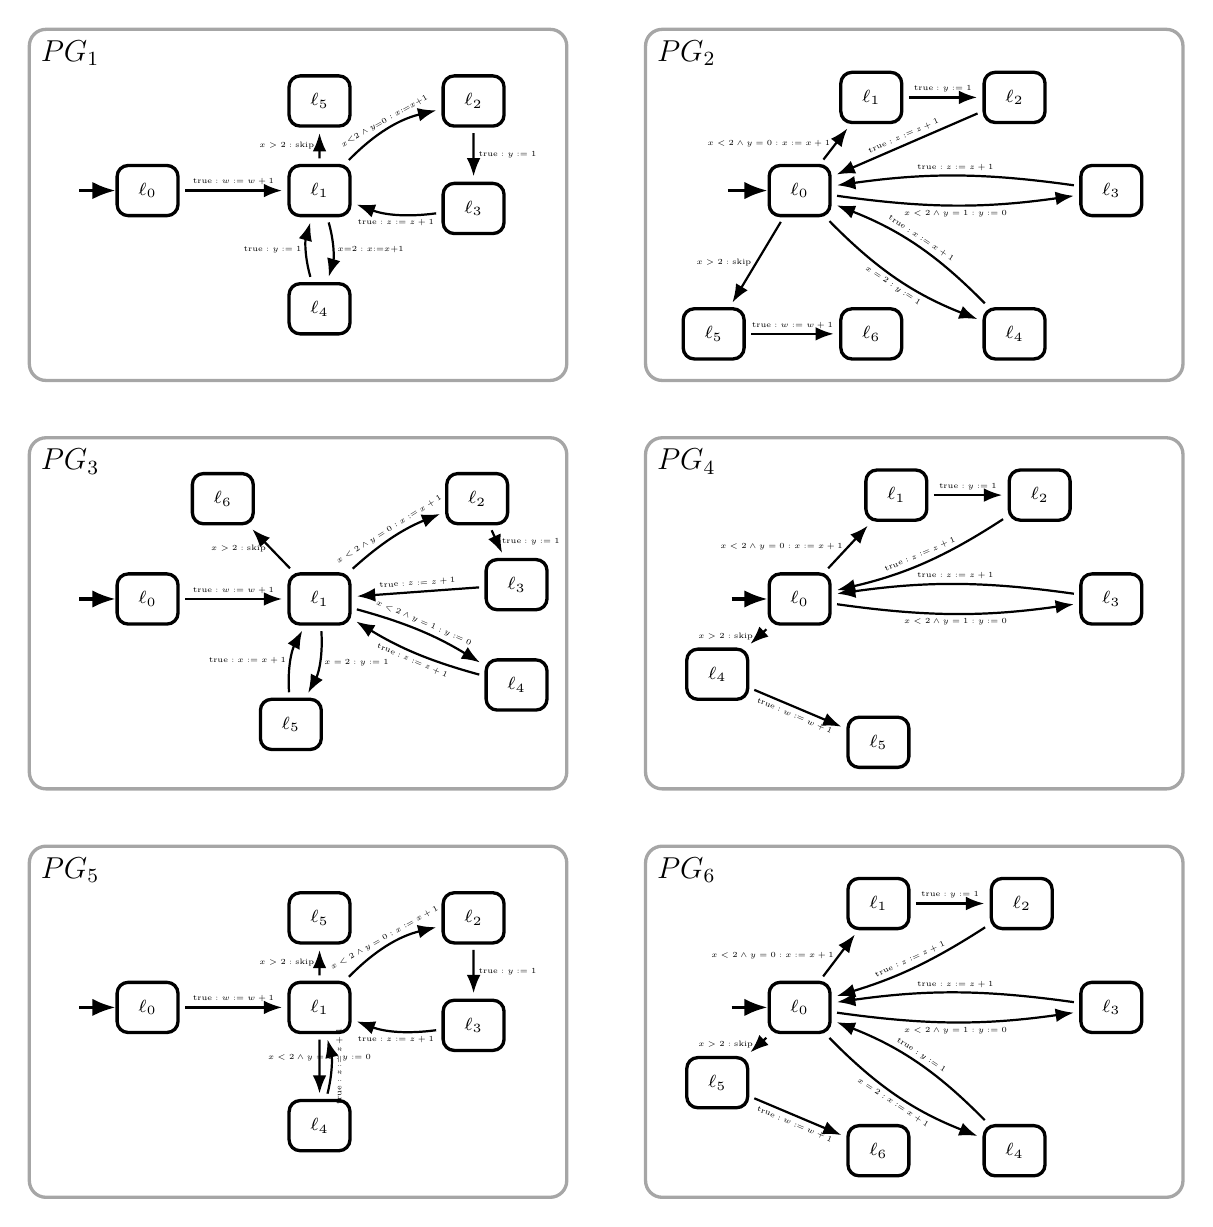
\begin{tikzpicture}[scale=0.91, transform shape]

  % -------------------------------------------------------------------
  % PG1
  % -------------------------------------------------------------------
  \begin{scope}[shift={(0,0)}]
    \node[state] (p10) at (0,0) {$\ell_0$};
    \node[state] (p11) at (2.4,0) {$\ell_1$};
    \node[state] (p12) at (4.55,1.25) {$\ell_2$};
    \node[state] (p13) at (4.55,-0.25) {$\ell_3$};
    \node[state] (p14) at (2.4,-1.65) {$\ell_4$};
    \node[state] (p15) at (2.4,1.25) {$\ell_5$};
    \initarrow{(-0.95,0)}{p10.west}
    \draw[edge]               (p10) to node[labelbox, above] {$\mathrm{true}:w:=w+1$} (p11);
    \draw[edge, bend left=16] (p11) to node[labelbox, above, sloped] {$x{<}2\land y{=}0:x{:=}x{+}1$} (p12);
    \draw[edge]               (p12) to node[labelbox, right] {$\mathrm{true}:y:=1$} (p13);
    \draw[edge, bend left=14] (p13) to node[labelbox, below] {$\mathrm{true}:z:=z+1$} (p11);
    \draw[edge, bend left=16] (p11) to node[labelbox, right] {$x{=}2:x{:=}x{+}1$} (p14);
    \draw[edge, bend left=16] (p14) to node[labelbox, left] {$\mathrm{true}:y:=1$} (p11);
    \draw[edge]               (p11) to node[labelbox, left] {$x>2:\mathrm{skip}$} (p15);
    \panel{(p10)(p11)(p12)(p13)(p14)(p15)}{pgonebox}{PG_1}
  \end{scope}

  % -------------------------------------------------------------------
  % PG2
  % -------------------------------------------------------------------
  \begin{scope}[shift={(8.6,0)}]
  \begin{scope}[shift={(.5,0)}]
    \node[state] (p20) at (0,0) {$\ell_0$};
    \node[state] (p21) at (1,1.3) {$\ell_1$};
    \node[state] (p22) at (3,1.3) {$\ell_2$};
    \node[state] (p23) at (4.35,0) {$\ell_3$};
    \node[state] (p24) at (3,-2) {$\ell_4$};
    \node[state] (p25) at (-1.2,-2) {$\ell_5$};
    \node[state] (p26) at (1,-2) {$\ell_6$};
    \initarrow{(-1.0,0)}{p20.west}
    \draw[edge]                (p20) to node[labelbox, left] {$x<2\land y=0:x:=x+1$} (p21);
    \draw[edge]                (p21) to node[labelbox, above] {$\mathrm{true}:y:=1$} (p22);
    \draw[edge]                (p22) to node[labelbox, above, sloped] {$\mathrm{true}:z:=z+1$} (p20);
    \draw[edge, bend right=8]  (p20) to node[labelbox, below] {$x<2\land y=1:y:=0$} (p23);
    \draw[edge, bend right=8]  (p23) to node[labelbox, above] {$\mathrm{true}:z:=z+1$} (p20);
    \draw[edge, bend right=12] (p20) to node[labelbox, below, sloped] {$x=2:y:=1$} (p24);
    \draw[edge, bend right=12] (p24) to node[labelbox, above, sloped] {$\mathrm{true}:x:=x+1$} (p20);
    \draw[edge]                (p20) to node[labelbox, left] {$x>2:\mathrm{skip}$} (p25);
    \draw[edge]                (p25) to node[labelbox, above] {$\mathrm{true}:w:=w+1$} (p26);
  \end{scope}
  \panel{(p20)(p21)(p22)(p23)(p24)(p25)(p26)}{pgtwobox}{PG_2}
  \end{scope}

  % -------------------------------------------------------------------
  % PG3
  % -------------------------------------------------------------------
  \begin{scope}[shift={(0,-5.7)}]
    \node[state] (p30) at (0,0) {$\ell_0$};
    \node[state] (p31) at (2.4,0) {$\ell_1$};
    \node[state] (p32) at (4.6,1.4) {$\ell_2$};
    \node[state] (p33) at (5.15,0.2) {$\ell_3$};
    \node[state] (p34) at (5.15,-1.2) {$\ell_4$};
    \node[state] (p35) at (2,-1.75) {$\ell_5$};
    \node[state] (p36) at (1.05,1.4) {$\ell_6$};
    \initarrow{(-0.95,0)}{p30.west}
    \draw[edge]                (p30) to node[labelbox, above] {$\mathrm{true}:w:=w+1$} (p31);
    \draw[edge, bend left=10]  (p31) to node[labelbox, above, sloped] {$x<2\land y=0:x:=x+1$} (p32);
    \draw[edge]                (p32) to node[labelbox, right] {$\mathrm{true}:y:=1$} (p33);
    \draw[edge, bend left=0]   (p33) to node[labelbox, above, sloped] {$\mathrm{true}:z:=z+1$} (p31);
    \draw[edge, bend left=8]   (p31) to node[labelbox, above, sloped] {$x<2\land y=1:y:=0$} (p34);
    \draw[edge, bend left=8]   (p34) to node[labelbox, below, sloped] {$\mathrm{true}:z:=z+1$} (p31);
    \draw[edge, bend left=16]  (p31) to node[labelbox, right] {$x=2:y:=1$} (p35);
    \draw[edge, bend left=16]  (p35) to node[labelbox, left] {$\mathrm{true}:x:=x+1$} (p31);
    \draw[edge]                (p31) to node[labelbox, left] {$x>2:\mathrm{skip}$} (p36);
    \panel{(p30)(p31)(p32)(p33)(p34)(p35)(p36)}{pgthreebox}{PG_3}
  \end{scope}

  % -------------------------------------------------------------------
  % PG4
  % -------------------------------------------------------------------
  \begin{scope}[shift={(8.6,-5.7)}]
  \begin{scope}[shift={(.5,0)}]
    \node[state] (p40) at (0,0) {$\ell_0$};
    \node[state] (p41) at (1.35,1.45) {$\ell_1$};
    \node[state] (p42) at (3.35,1.45) {$\ell_2$};
    \node[state] (p43) at (4.35,0) {$\ell_3$};
    \node[state] (p44) at (-1.15,-1.05) {$\ell_4$};
    \node[state] (p45) at (1.1,-2.0) {$\ell_5$};
    \initarrow{(-0.95,0)}{p40.west}
    \draw[edge]                (p40) to node[labelbox, left] {$x<2\land y=0:x:=x+1$} (p41);
    \draw[edge]                (p41) to node[labelbox, above] {$\mathrm{true}:y:=1$} (p42);
    \draw[edge, bend left=10]  (p42) to node[labelbox, above, sloped] {$\mathrm{true}:z:=z+1$} (p40);
    \draw[edge, bend right=8]  (p40) to node[labelbox, below] {$x<2\land y=1:y:=0$} (p43);
    \draw[edge, bend right=8]  (p43) to node[labelbox, above] {$\mathrm{true}:z:=z+1$} (p40);
    \draw[edge]                (p40) to node[labelbox, left] {$x>2:\mathrm{skip}$} (p44);
    \draw[edge]                (p44) to node[labelbox, below, sloped] {$\mathrm{true}:w:=w+1$} (p45);
  \end{scope}
    \panel{(p40)(p41)(p42)(p43)(p44)(p45)}{pgfourbox}{PG_4}
  \end{scope}

  % -------------------------------------------------------------------
  % PG5
  % -------------------------------------------------------------------
  \begin{scope}[shift={(0,-11.4)}]
    \node[state] (p50) at (0,0) {$\ell_0$};
    \node[state] (p51) at (2.4,0) {$\ell_1$};
    \node[state] (p52) at (4.55,1.25) {$\ell_2$};
    \node[state] (p53) at (4.55,-0.25) {$\ell_3$};
    \node[state] (p54) at (2.4,-1.65) {$\ell_4$};
    \node[state] (p55) at (2.4,1.25) {$\ell_5$};
    \initarrow{(-0.95,0)}{p50.west}
    \draw[edge]               (p50) to node[labelbox, above] {$\mathrm{true}:w:=w+1$} (p51);
    \draw[edge, bend left=16] (p51) to node[labelbox, above, sloped] {$x<2\land y=0:x:=x+1$} (p52);
    \draw[edge]               (p52) to node[labelbox, right] {$\mathrm{true}:y:=1$} (p53);
    \draw[edge, bend left=14] (p53) to node[labelbox, below] {$\mathrm{true}:z:=z+1$} (p51);
    \draw[edge]               (p51) to node[labelbox, above] {$x<2\land y=1:y:=0$} (p54);
    \draw[edge, bend right=14](p54) to node[labelbox, below, sloped] {$\mathrm{true}:z:=z+1$} (p51);
    \draw[edge]               (p51) to node[labelbox, left] {$x>2:\mathrm{skip}$} (p55);
    \panel{(p50)(p51)(p52)(p53)(p54)(p55)}{pgfivebox}{PG_5}
  \end{scope}

  % -------------------------------------------------------------------
  % PG6
  % -------------------------------------------------------------------
  \begin{scope}[shift={(8.6,-11.4)}]
  \begin{scope}[shift={(.5,0)}]
    \node[state] (p60) at (0,0) {$\ell_0$};
    \node[state] (p61) at (1.1,1.45) {$\ell_1$};
    \node[state] (p62) at (3.1,1.45) {$\ell_2$};
    \node[state] (p63) at (4.35,0) {$\ell_3$};
    \node[state] (p64) at (3,-2) {$\ell_4$};
    \node[state] (p65) at (-1.15,-1.05) {$\ell_5$};
    \node[state] (p66) at (1.1,-2.0) {$\ell_6$};
    \initarrow{(-0.95,0)}{p60.west}
    \draw[edge]                (p60) to node[labelbox, left] {$x<2\land y=0:x:=x+1$} (p61);
    \draw[edge]                (p61) to node[labelbox, above] {$\mathrm{true}:y:=1$} (p62);
    \draw[edge, bend left=8]   (p62) to node[labelbox, above, sloped] {$\mathrm{true}:z:=z+1$} (p60);
    \draw[edge, bend right=8]  (p60) to node[labelbox, below] {$x<2\land y=1:y:=0$} (p63);
    \draw[edge, bend right=8]  (p63) to node[labelbox, above] {$\mathrm{true}:z:=z+1$} (p60);
    \draw[edge, bend right=12] (p60) to node[labelbox, below, sloped] {$x=2:x:=x+1$} (p64);
    \draw[edge, bend right=12] (p64) to node[labelbox, above, sloped] {$\mathrm{true}:y:=1$} (p60);
    \draw[edge]                (p60) to node[labelbox, left] {$x>2:\mathrm{skip}$} (p65);
    \draw[edge]                (p65) to node[labelbox, below, sloped] {$\mathrm{true}:w:=w+1$} (p66);
  \end{scope}
    \panel{(p60)(p61)(p62)(p63)(p64)(p65)(p66)}{pgsixbox}{PG_6}
  \end{scope}

\end{tikzpicture}
\end{document}
